\section{Chapter Overview}
This chapter will cover the network implemented in the course of the project, beginning with the individual \ac{ADPLL}'s composition. A number of attributes for each design will be used to analyse and compare their performance. The impact of some minor architectural changes will also be covered, before the implementation of test network will be described. This chapter will also highlight some pitfalls encountered in the process. The \ac{HDL} Verilog was selected for use in this project due to my prior exposure to that language.

\section{\acs{ADPLL} Architectures}
Three different architectures of \ac{ADPLL} were implemented in this project for the purposes of testing, and re-use in the future within the research team in \acl{UCD}. Between each design a number of blocks remain constant, as only a single instance of that block was implemented, as variation its design would have negligible impact on the final system. These blocks were the error combiner and frequency divider. The loop filter was implemented both using fractional and integer arithmetic, but as the exact same calculation was performed in both cases there was no impact on the output of the module.

The three architectures chosen for implementation represent a progression from entirely an \ac{FPGA} clock driven system to an \ac{ADPLL} with all components asynchronous with respect to that clock. Therefore the first \ac{ADPLL} design features a clocked oscillator and phase detector, specifically the linear frequency design mentioned in Chapter \ref{chap:3} and the clocked phase detector using a state machine and a bi-directional counter. Skipping over Design 2, the final design used was asynchronous in totality, featuring the \acl{RO} and SigNum/\ac{TDL} phase detector. Design 2 sat between these two, using the \ac{RO} as its oscillator, but retained the clocked phase detector seen in Design 1.

The extensibility of the end product of this project was to the forefront during the design process. Whilst, apart from frequency, there were no guidelines as to what the system should resemble and a number of attributes could be chosen arbitrarily, a future user of this platform could have entirely different requirements or specifications. As such each block was implemented in such a way that changing the number of bits used for a certain signal, the target frequency or swapping between different blocks could be done with the sole requirement of changing Verilog \texttt{localparam}\footnote{A \texttt{localparam} is a constant that cannot be modified in a module instance statement \cite{hdlworks}}s in the module \footnote{Module is the Verilog term for a number of logic elements grouped to provide a certain functionality} in which change was made, which would then propagate to any sub-modules affected. Starting the design process with this in mind was a major benefit at later stages when frequent modifications were being made to test their impact, or when changing between \ac{ADPLL} designs.

\subsection{Generic Components}
As mentioned in the chapter overview, a number of components were used in all \ac{ADPLL}s implemented, as changes in their design would not impact the overall system.
\subsubsection{Error Combiner}
The error combiner in this design had a number of requirements in order to be suitable for use in both a single \ac{ADPLL} as well as a network operating in both uni- and bi-directional modes, alongside modifications which would change the widths of the error signals requiring averaging. The module was implemented on the basis that the \ac{LF} input width would be identical to the phase detector output width.

The error combiner was designed to take in up to four error signals, all of an identical width which defaults to eight, and four weights to apply in the summation process. A weighted summation is performed by multiplying each error signal by the weight and adding the results together. Regardless of the number of input error signals, a division by four is then performed in order to compute the average error, done by shifting the value right by two. In a \ac{HDL}, unlike C programming or similar, a shift requires no computation and is instead implemented by performing a part-selection. As all error signals are two's complemented signed integers, the error combination process is also carried out using signed values. The code implementing the error combiner can be found in \textsc{ErrorCombiner.v}, attached in Appendix \ref{adx:code} Listing \ref{lst:error_combiner}.

\subsubsection{Frequency Divider}
The frequency divider is implemented using ``Divider 2'' from Chapter \ref{chap:3}, as only divisions ratios of 2, 4 and 8 were selected for use in the testing process. For ease of testing, the divider had outputs representing each of these division ratios simultaneously, which could be multiplexed between at runtime if so desired. A fourth output passed the input through unmodified, allowing for the divider to be removed without regeneration of the \ac{FPGA} configuration.
\begin{figure}[h]%
	\centering
	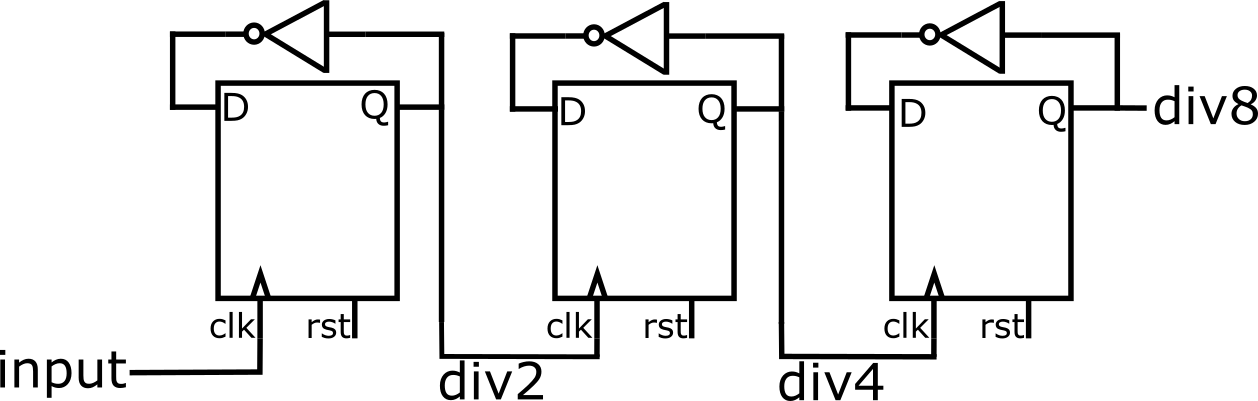
\includegraphics[width=0.6\textwidth]{../divider2}
	\caption[Frequency divider \ac{RTL} diagram]{Frequency divider \ac{RTL} diagram.}
	\label{fig:divs_iompl}
\end{figure}

\subsubsection{Loop Filter}
Two \acl{LF}s were implemented, both as \ac{IIR} filters. \ac{FIR} was dismissed due to the extra hardware required to implement the calculations within a single clock cycle, as the \ac{LF} is clocked using the oscillator output, and the greater difficulty of gain adjustment compared to an \ac{IIR}. Clocking on using the generated signal ensures that the discrete time integration is only carried out once per phase comparison. A pitfall that may be encountered implementing an \ac{ADPLL} featuring a divider is not clocking the module on the divided clock, which will result in the integration being carried out at the oscillator output frequency.

Each of integer and fixed-point arithmetic were used to implement a filter respectively, however both designs are interchangeable as they perform the integration identically, given the same proportional and integral gains. All testing was carried out using integer arithmetic, as in Figure \ref{fig:integer_lf}, however the interchangeability will be confirmed later in this chapter, in Section \ref{section:minor_variations}. Additionally the \ac{LF} supports variation of both \acs{ki} and \acs{kp} at runtime, however, if a static value is desired the runtime variation may be disabled using a \texttt{parameter}\footnote{Parameters are constant values that may be changed at compile time, or in the module instance statement \cite{hdlworks2}}.
\begin{figure}[h]%
	\centering
	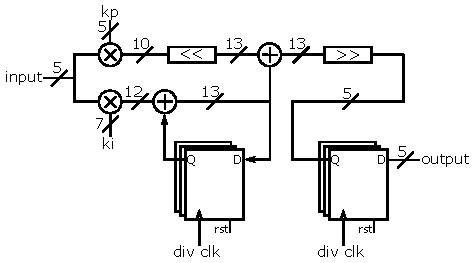
\includegraphics[width=0.8\textwidth]{../integer_lf} 
	\caption[\acl{LF} implemented using integer arithmetic \ac{RTL} diagram]{\acl{LF} implemented using integer arithmetic \ac{RTL} diagram (signal widths using default values).}
	\label{fig:integer_lf}
\end{figure}

Figure \ref{fig:integer_lf} contains an \ac{RTL} diagram describing the implementation. Important to note is the shift applied to the result of the multiplication by \acs{kp} which, as the integration is performed with a larger width to avoid accumulator overflow, preserves the intended relationship between proportional and integral gains.
The Verilog implementation of the \ac{LF} using integer arithmetic can be found in \textsc{LoopFilter.v}, attached in Appendix \ref{adx:code} Listing \ref{lst:loop_filter}.

\subsection{\acs{ADPLL} Design 1}
\subsubsection{Oscillator}
\subsubsection{Phase Detector}

\subsection{\acs{ADPLL} Design 2}
\subsubsection{Oscillator}
\subsubsection{Phase Detector}

\subsection{\acs{ADPLL} Design 3}
\subsubsection{Oscillator}
\subsubsection{Phase Detector}


\section{\acs{ADPLL} Characterisation}

\section{Minor Variations}\label{section:minor_variations}

\section{\acs{ADPLL} Network Implementation}
\subsection{2x2 Network}
\subsection{3x3 Network}
